\section{障害物認識}
自己位置とゴール座標が分かればロボットが進むべき経路を計算できる。
ただし、これだけでは現実にある衝突してはいけない障害物を考慮していない。
LiDARなどのセンサを使って障害物を認識し、それを地図に反映させることで障害物を考慮した経路を計算することができる。

多くのロボットでは、2DLiDARを障害物に使用している。
2DLiDARを使用すると、ロボットに設置した高さの平面でしか障害物を認識することができない。
それによって、背の低い障害物が認識できなかったり、パイロンなどのように地面に向かって太くなる形状のものは本来より小さな障害物として認識したりすることがある。
また、坂道のようにロボットが傾いている時は、地面を障害物として認識することがある。
2DLiDARは工夫しないと、認識したい障害物を見逃したり、地面のような障害物でないものも障害物として認識することがある。

Abudori Lab.チームでは、3DLiDARを使うことで、小さな障害物を認識し、坂道などの地面はアルゴリズムで除外することで、上記の問題を回避した。
このアルゴリズムはOSSでobstacle-cloud-to-scan\cite{obstacle}として公開している。

\subsection{obstacle-cloud-to-scan}
このパッケージは、3DLiDARでロボット直近の3次元点群を取得し、障害物のみを抜き出し2DLiDARのScanとして出力する。

簡単な手順としては以下の通りだ。
\begin{itemize}
    \item 点群をダウンサンプリングする
    \item LiDAR点群の傾きを設置角度分回転し水平にする
    \item 法線を各点ごとに計算する
    \item 法線ベクトルから垂直に近いもののみを抜き出す
    \item 垂直に近い点群をscanに変換する
\end{itemize}

法線ベクトルに注目することで、坂道や乗り越えられる小さな段差は障害物と認識しない判断ができた。
壁や大きな段差は、法線ベクトルが水平方向に向くため障害物として認識することができた。

障害物と坂道を判断する計算を単純にするために、法線のZ方向で閾値で区切った。
つくばチャレンジでは、斜度25度に傾いた時のZ方向の高さを閾値に、それよりもZの値が小さいものを障害物が映った点群と判断した。
この閾値処理のみで、細い鉄パイプやパイロンの根本、パイロンにかかった棒も障害物として判定できた。
苦手な物体として、背のひくい水平な障害物は検出することが難しい。
身近にあるものとしては、平台車や高さが20cm程度のダンボールなどが挙げられる。
幸い、つくばチャレンジの環境にはなかったため、障害物認識で苦戦することはなかった。

出力した点群をOSSのpointcloud\_to\_laserscan\cite{laserscan}パッケージに入力し、2DLiDARのscanトピックに変換した。
このScanトピックをNavigation2に入力することで、広く使われる2DLiDARのサンプルをそのまま動かすことができた。

\begin{figure}[t]
    \centering
    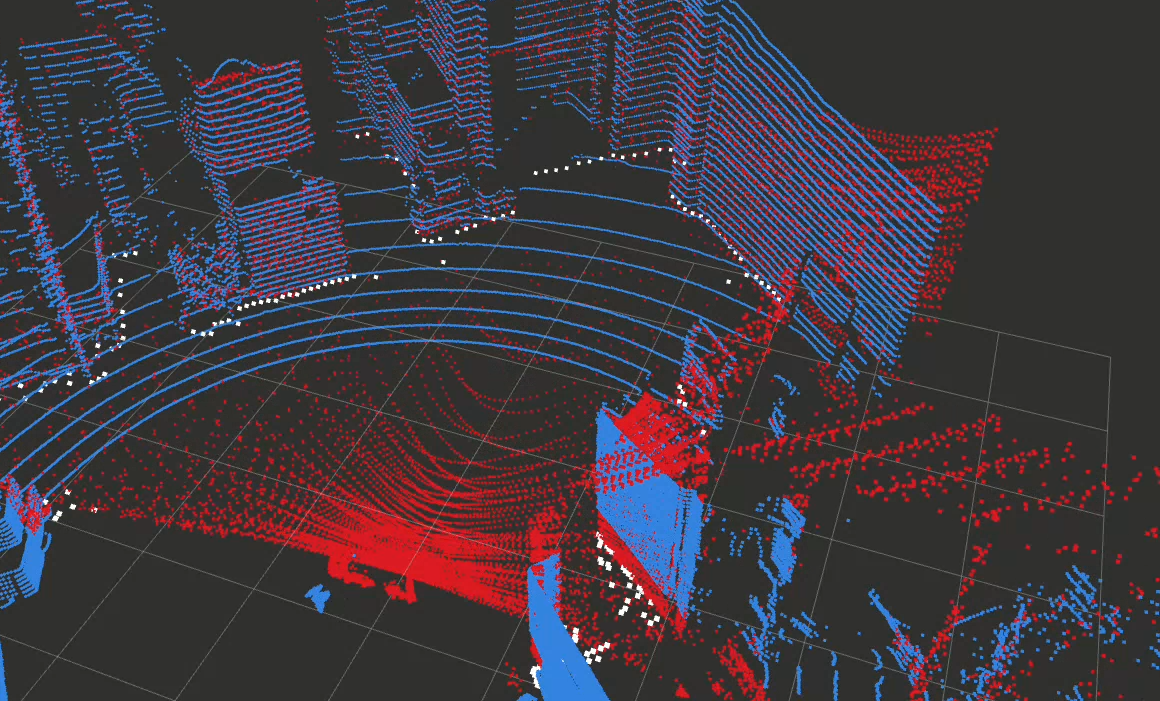
\includegraphics[height=5cm]{fig/obstaclescan.png}
    \caption{左の図}
    \label{fig:obstaclescan}
\end{figure}